\documentclass{article}

\usepackage{hyperref}
\usepackage{titlesec}
\usepackage{titling}
\usepackage[margin=0.2in]{geometry}
\usepackage{graphicx}
\usepackage{multicol}
\titleformat{\section}
{\large\uppercase}
{}
{0em}
%{}[\titlerule]
{}
%[runin]
\titleformat{\subsection}
{\bfseries}
{}
{1em}
{}[]

\renewcommand{\maketitle}{
    \begin{flushleft}        
        {\huge\rmfamily
        \theauthor}\newline
        \vspace{0.1em}
        \textit{Email: sahilsainisalaria@gmail.com }  \newline  
        \textit{Contact: +91 9682663655 }  \newline 
        \textit{Address: Jammu, Jammu \& Kashmir }  \newline 
        % \textit{ Website:  \href{https://sahil1515.github.io/My-Website/}{My Profile}}\newline 
        \textit{ \href{https://github.com/sahil1515}{GitHub}}  \newline 
    \end{flushleft}
}

\titlespacing*{\subsection}
{0em}{0.25em}{0.1em}

%%%%%%%%%%%%%%%%%%%%%%%%%%%%%%%%

\begin{document}

\begin{multicols}{2}
    \title{Resume}
    \author{Sahil Saini Salaria}
    \maketitle

    % \begin{flushright}
    %     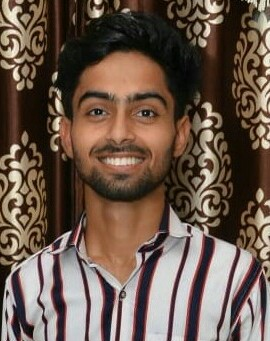
\includegraphics[height=3cm]{../images/Sahil.jpeg}
    % \end{flushright}

\end{multicols}


\section{\underline{Work Experience}}

\subsection{\textbf{Backend Engineer - Intern}
    \textmd{- FOLK Developers (Nov'20 - Ongoing)}\newline
    \textmd{- Worked on Backend Development with Python and Google Cloud Platform and its tools such as Firebase, Cloud Functions. }\newline
    \textmd{- Built “Serverless” RESTful APIs with Cloud Functions, Firestore and Flask}\newline
    \textmd{- Deployed different Microservices on Google App Engine}\newline
    \textmd{- Created GCP Pub/Sub topics for sending notifications to the subscribers.}\newline
    \textmd{- Created Cloud functions using different triggers such as HTTP, Firestore, Firebase Authentication, Pub/Sub}\newline
    \textmd{- Tested API endpoints using Postman, Requests Library and Cloud Function testing}\newline
    \textmd{- Developed the sign-up and login system that authenticates user using Firebase Authentication}\newline
}

% Education
\section{\underline{Education}}

\subsection{\textbf{Bachelor of Technology (B.Tech), Computer Science \& Engineering}\newline
    \textmd{Manipal Institute of Technology, Manipal --  2018 - 2022 -- CGPA: 8.30/10}}

\subsection{\textbf{Senior Secondary (XII), Science}\newline
    \textmd{ Shiksha Niketan Higher Secondary, Jammu -- Year of completion: 2018 --  Percentage: 93.00\%}}

% \subsection{\textbf{Secondary (X),Science}\newline 
% \textmd{Fatima Covent, Jammu -- Year of completion: 2016 -- Percentage: 90.20\%}}

\section{\underline{Projects}}





\subsection{\textbf{Geocoding and Distance Measurement with GeoPy:}
    % \newline
    \textmd{Used GeoPy to retrieve a user's location and identify the user's nearby centers from a database and assign the center so that it can be reflected in the profile.}}

\subsection{\textbf{Routing System}
    \textmd{Used Smopy, Networksx and GeoPy to develop a routing system that returns a route from given source and destination. Also used Google Maps JavaScript API to pinpoint current location in Google Maps. }}

\subsection{\textbf{Personal Voice Assistant}
    \textmd{Implemented a voice assistant that can open up an application,
        search Google, Wikipedia and YouTube about the given query, solve mathematical problems, etc }}

\subsection{\textbf{Web Scrapper:}
    \textmd{Developed a Web Scrapper using Python to scrape the reviews of a product from some commercial website.
        Stored that data using MongoDB and then displayed using Flask.}}

\subsection{\textbf{Covid-19 Worldwide Data}
    \textmd{Built Covid Statistics website using Django that uses Rapid API to retrieve the live data.}}

\subsection{\textbf{Boston Housing Price Prediction:}
    \textmd{Applied Data-preprocessing,Data Visualization and Machine Learning techniques to create a
        Linear Regression model to predict the house prices in Boston,Massachusetts. } }

\subsection{\textbf{Finland Labs and IIT Roorkee - ML \& AI Using Covid 19 Virus Data Analysis Workshop:}
    \textmd{Applied Data Pre-processing, Visualization and Machine Learning techniques to make the predictions how the cases will increase/decrease in the country. } }

% \subsection{\textbf{Data Exchange in Heterogeneous Systems(Collaborative project):}
%     \textmd{The objective of this project is to experience the real
%         world problem of data exchange in a automatic fashion between different generations
%         of applications.So we are trying to prove $sin^2(x) + cos^2(x)=1$ } 
%     \textmd{Here we consider three systems communicating the data.}
% }

% Courses
\section{\underline{Courses}}


\subsection{\textbf{Machine Learning using Python Online-Project-based-course }
    \textmd{- Skyfi Labs}}

\subsection{\textbf{Data Analysis and Data Visualization}
    \textmd{- Ineuron}}

\subsection{\textbf{Python Programming}
    \textmd{- Ineuron}}

% \subsection{\textbf{Statistics for Data Science}
%     \textmd{- Ineuron}}

% \subsection{\textbf{ML and AI using COVID-19 virus Data Analysis workshop}
% \textmd{- Finland Labs}}

\subsection{\textbf{Accessing web Data using Python}
    \textmd{- Coursera}}

\subsection{\textbf{Google Crash Course on Python}
    \textmd{- Coursera}}

\subsection{\textbf{Python by University of Michigan}
    \textmd{- Coursera}}


% Skills
\section{\underline{Skills}}

\subsection{\textbf{Programming Languages:}\textmd{Fluent in C/C++, Python }}
\subsection{\textbf{Web Development :}\textmd{- HTML, CSS, JavaScript,Jquery, React, Django and Flask}}
\subsection{\textbf{Data Pre-processing and Data Analysis :}\textmd{Pandas, Numpy, Matplotlib, Seaborn }}
\subsection{\textbf{Database Management Systems :}\textmd{ Oracle SQL, Firestore, MongoDB }}
\subsection{\textbf{Familiar with :}\textmd{ Java, SQL, {\LaTeX},Linux Shell Scripting }}




% \textbf{Libraries and Frameworks:}\newline
% \textbf{Python:}\textmd{- Numpy, Pandas,Scikit-Learn,Matplotlib,seaborn and some others.}
% \textbf{C++:}\textmd{- Standard Template Library(STL)\newline}
% \textbf{Java:}\textmd{- JavaFX GUI.}\newline

% \subsection{\textbf{Others:}\textmd{}}


% Skills



\section{\underline{Leadership/Involvement}}
\subsection{% \textmd{-Member of ACM college club. }\newline
    % \textmd{-Member of College and university athletics teams. }\newline
    % \textmd{-Interviewed second year students for ACM club recruitment. }\newline
    % \textmd{-Part time tutor for Secondary students. }\newline
    \textmd{-Vice-Captain of college athletics team and member of organising team of the Manipal Marathon.}\newline
    \textmd{-Awarded with Best Athlete Award in Revels'19, the National Cultural and Sports Fest of MIT. Won many other medals in Athletics. }\newline
    \textmd{-PMSSS, AICTE scholarship holder for graduation.}}

%     Languages
% \section{\underline{Languages}}

%     \subsection{\textbf{English, Hindi, Punjabi, Dogri}}

% \end{document}
\end{document}




